\chapter{Thermo with Push } \label{chapter:Thermo with Push}

We combine FacePush with Thermo to improve the user experience in the applications by controlling the temperature increase and decrease. In the boxing application, we use heat to simulate the burning sensation when the user is heavy struck by a blow. On the other hand, use cold to simulate the cold feeling when encountering ocean currents during a dive. Next, we'll describe the updated application and how our system hardware can be combined with Thermo.

\section{Hardware Combined}

\begin{figure}[hp]
    \begin{center}
        \begin{tabular}{@{\hspace{0.1cm}}c}
           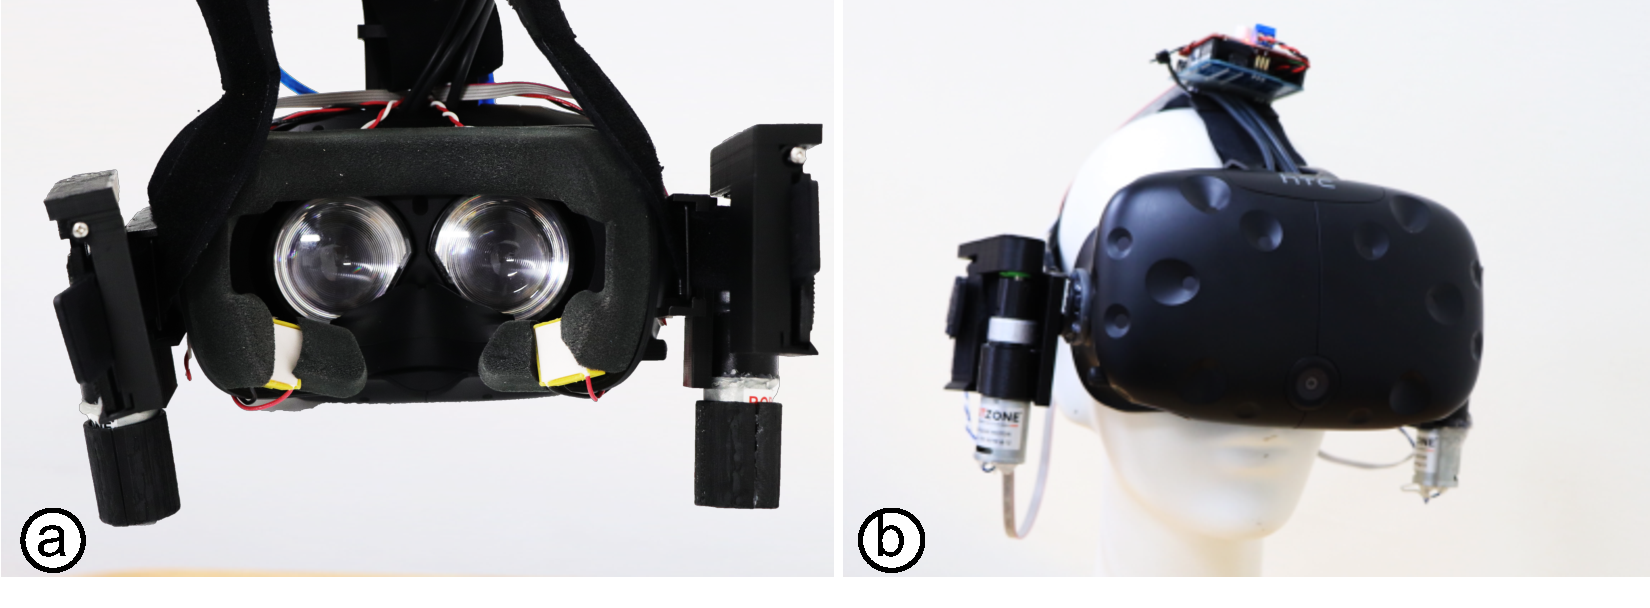
\includegraphics[width=1\textwidth]{figures/ThermoFacePush.pdf}
        \end{tabular}
        \captionof{figure}{(a) Seen from inside (b) A front view of the FacePush with Thermo}
        \label{fig:ThermoFacePush Overview}
    \end{center}
\end{figure}

The prototype is shown in Figure \ref{fig:ThermoFacePush Overview}(a-b). Two 2cm x 2cm peltier modules (Figure \ref{fig:PiltierModule} (a-b))\footnote{\url{https://ppt.cc/fT4F7x}} with a power supply rated at 8.6V, 6A were attached to the Vive HMD using a custom 3D printed rig.  When FacePush is worn by a user, the peltier modules are in contact with the two locations cheekbone (left and right).  When the HMD is worn, these locations are in constant contact with the user’s face. Each peltier moduleis driven by a external motor driver (VNH2SP30-E) and an Arduino UNO board interfaced with a PC using a USB serial connection running at a 115200 baudrate. To improve heat dissipation, we installed a copper heat sink (1.2 cm x 1.3 cm x 0.5 cm) behind the Peltier module (Figure \ref{fig:PiltierModule}(b)).


\begin{figure}[hp]
    \begin{center}
        \begin{tabular}{@{\hspace{0.1cm}}c}
           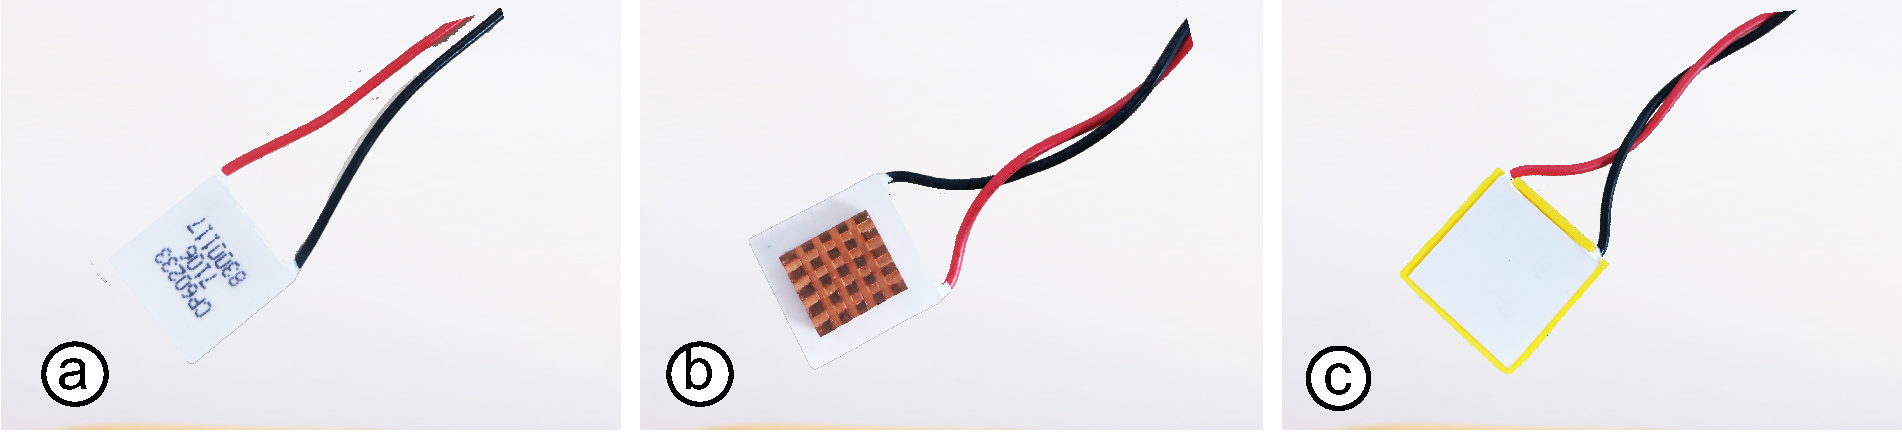
\includegraphics[width=1\textwidth]{figures/PiltierModule.pdf}
        \end{tabular}
        \captionof{figure}{(a) A front view of the piltier module (b) A back view of the piltier module (c) Combined with 3D printed rig}
        \label{fig:PiltierModule}
    \end{center}
\end{figure}

\section{Updated Applications}

We also updated the applications. In boxing applications(Figure \ref{fig:UpdatedApplication} (a)), when the opponent punches heavily, the Peltier module will provide thermal 
feedback to the user. Let the user feel the power of the punch is extraordinary, resulting in a different experience. Each time the heat feedback comes with a focus on the punch, and lasts for 1 second, ensuring that every user can feel it. 

On the other hand, in the diving application(Figure \ref{fig:UpdatedApplication} (b)), we use the peltier modules to generate cold. Every cold feeling lasts for 1 second and occurs every 20 seconds. In this way, the feeling of the ocean current passing through the face is simulated to enhance the realism of the user during the experience.

\begin{figure}[b!]
    \begin{center}
        \begin{tabular}{@{\hspace{0.1cm}}c}
           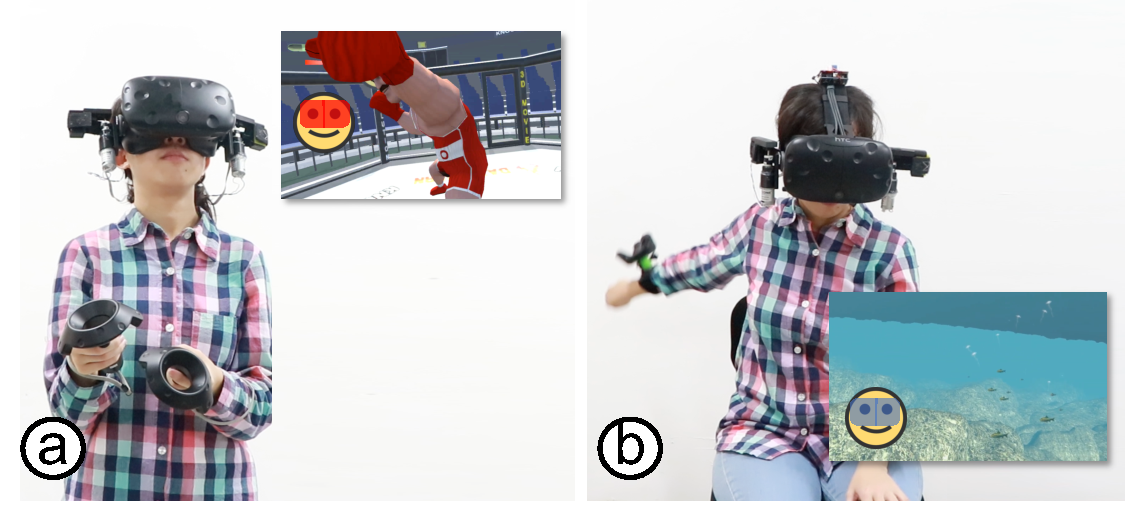
\includegraphics[width=1\textwidth]{figures/UpdatedApplication.pdf}
        \end{tabular}
        \captionof{figure}{(a) Boxing with heat (b) Diving with cold}
        \label{fig:UpdatedApplication}
    \end{center}
\end{figure}
